\documentclass[10pt,twocolumn,letterpaper]{article}

\usepackage{iccv}
\usepackage{times}
\usepackage{epsfig}
\usepackage{graphicx}
\usepackage{amsmath}
\usepackage{amssymb}

%%addied by shubham
\usepackage{caption}
\usepackage{booktabs}
\usepackage{multirow}
\usepackage{ctable}
\newcommand{\overbar}[1]{\mkern 1.5mu\overline{\mkern-1.5mu#1\mkern-1.5mu}\mkern 1.5mu}
\newcommand*\samethanks[1][\value{footnote}]{\footnotemark[#1]}
\usepackage{subcaption}
% \usepackage{subcaption}
%%end added by shubham %%

% Include other packages here, before hyperref.

% If you comment hyperref and then uncomment it, you should delete
% egpaper.aux before re-running latex.  (Or just hit 'q' on the first latex
% run, let it finish, and you should be clear).
\usepackage[pagebackref=true,breaklinks=true,letterpaper=true,colorlinks,bookmarks=false]{hyperref}

% \iccvfinalcopy % *** Uncomment this line for the final submission

\def\iccvPaperID{2171} % *** Enter the ICCV Paper ID here
\def\httilde{\mbox{\tt\raisebox{-.5ex}{\symbol{126}}}}

% Pages are numbered in submission mode, and unnumbered in camera-ready
\ificcvfinal\pagestyle{empty}\fi
\begin{document}

%%%%%%%%% TITLE
\title{High Accuracy Face Geometry Capture using a Smartphone Video}

\author{First Author\\
Institution1\\
Institution1 address\\
{\tt\small firstauthor@i1.org}
% For a paper whose authors are all at the same institution,
% omit the following lines up until the closing ``}''.
% Additional authors and addresses can be added with ``\and'',
% just like the second author.
% To save space, use either the email address or home page, not both
\and
Second Author\\
Institution2\\
First line of institution2 address\\
{\tt\small secondauthor@i2.org}
}

% \maketitle
%\thispagestyle{empty}

\twocolumn[{%
\renewcommand\twocolumn[1][]{#1}%
\vspace{-1em}
\maketitle
\vspace{-1em}
\begin{center}
   \centering 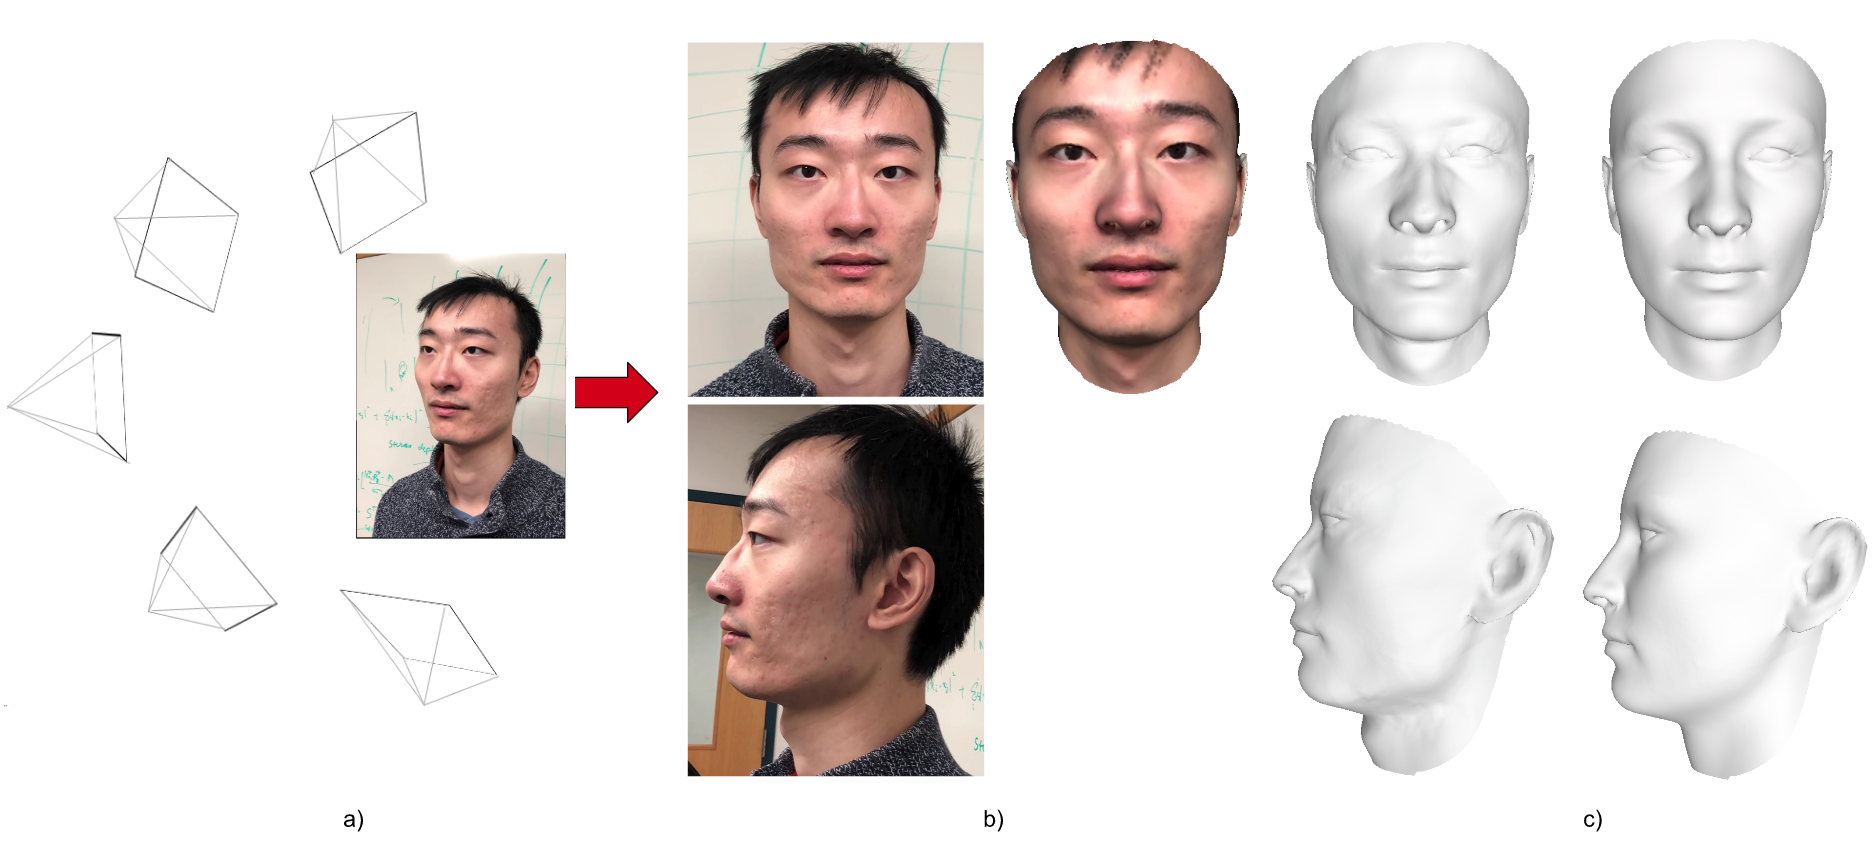
\includegraphics[width=\textwidth]{../images/cover_chaoyang.png} \captionof{figure}{a) Our method uses a single video clip of a subject taken in an unconstrained environment to reconstruct a highly accurate mesh of the face geometry. b) Our textured mesh side-by-side with input rgb image c) Our method (left) compared to the state-of-the-art method of \cite{hernandez2017accurate}(right), front and profile view.}
   \label{cover}
\end{center}%
}]


%%%%%%%%% ABSTRACT
\begin{abstract}
   The ABSTRACT is to be in fully-justified italicized text, at the top
   of the left-hand column, below the author and affiliation
   information. Use the word ``Abstract'' as the title, in 12-point
   Times, boldface type, centered relative to the column, initially
   capitalized. The abstract is to be in 10-point, single-spaced type.
   Leave two blank lines after the Abstract, then begin the main text.
   Look at previous ICCV abstracts to get a feel for style and length.
\end{abstract}

%%%%%%%%% BODY TEXT
\section{Introduction}


Reconstructing faces has been a problem of great interest in computer vision and graphics with applications in a wide variety of domains, ranging from animation \cite{ichim2015dynamic}, entertainment \cite{saito2016real}, genetics, bio-metrics, and more recently, augmented and virtual reality. Despite the long body of work, 3D face reconstruction still remains an open and challenging problem, primarily because the high level of detail required owing to our sensitivity to facial features. Even slight anomalies in the reconstructions can make the output look unrealistic and hence, accuracy of reconstructed face models is of utmost importance.


The seminal work of Beeler \etal \cite{beeler2010high} used a studio setup of cameras to capture face geometry accurately. Since then, a variety of work has focused on using Photometric stereo or Multi-view stereo techniques in studio settings for face reconstruction and performance capture \cite{cao2018sparse, fyffe2017multi}. 
Although accurate in their reconstructions, these studio setups are not trivial to setup, typically requiring a calibrated camera setup along with controlled lighting and backgrounds. This makes them infeasible for capturing `in-the-wild' subject faces in unconstrained settings, for instance an end user of a virtual reality app. For the purposes of animation or modeling, accurate 3D scans can be obtained from structured light or laser scanners, which are often prohibitively expensive, typically costing tens of thousands of dollars. 

To tackle the problem of unconstrained 3D face reconstruction, the community has mostly relied on three-dimensional morphable models (3DMMs)~\cite{blanz1999morphable}. 3DMMs are low-dimensional linear sub-spaces of faces typically constructed using a small set of ground truth 3D scans that enable rapid approximation of face geometry, typically through a combination of appearance based and landmark based optimization. In recent years, there has been a lot of interest in using deep neural nets to fit morphable models using a single image. However, single view depth estimation is a fundamentally ill-posed problem. Coupled with the reliance on synthetic data, generalization to in-the-wild images is often a concern for these methods. Often, while the results are visually appealing with texture, the reconstructions suffer from high geometric inaccuracies.

With the limited availability of 3D data for faces, using geometric cues from multiple views to improve accuracy of reconstruction becomes necessary. Previous work has shown that a single template or 3DMM can be optimized using constraints from multiple views, using techniques like photometric stereo \cite{roth2015unconstrained} or advances in automatic keypoint detection \cite{huber2016multiresolution}.
Recently, Hernandez \etal \cite{hernandez2017accurate} proposed an elegant multi-view constrained structure-from-motion scheme that explicitly optimized the coefficients of a 3DMM shape to recover face geometry. However, the output still remains constrained to the underlying training data and low capacity of the 3DMM. This greatly limits its expressivity, and is particularly undesirable for medical or bio-metric usage. 


In this work, we attempt to answer the question ``What's the most accurate reconstruction an end-user can obtain, without needing access to special equipment or studio setups?". To this end, we propose a pipeline for highly accurate yet robust face geometry capture, requiring nothing but a smartphone. We leverage recent advances in the fields of object and keypoint detection, direct methods for visual SLAM, and higher frame-rate capture functionality available on modern smartphones to propose a pipeline that achieves state-of-the-art geometric accuracy among unconstrained face reconstruction techniques.

Our major contributions are as follows:
 \begin{itemize}
     \item  A principled reconstruction pipeline that takes a single video of a subject's face and reconstructs their face geometry with high fidelity. The reconstructed meshes are in dense semantic correspondence without being constrained to any model subspace, making them ideal for usage in downstream tasks like animation, printing, genetic analysis/modeling, biometrics etc. We make the code public, allowing anyone to be able to obtain accurate reconstructions of faces
     \item A collected dataset of 200 high-frame-rate  sequences of 100 individuals, where we collect two sequences per subject, under varying lighting conditions.
 \end{itemize}

\section{Prior Work}
Prior work on 3D Face Reconstruction is substantially large and a complete literature review is out of scope for the paper. Here, we talk about about some of the works closely related to ours.

\noindent \textbf{SfM based Multi-view Reconstruction.} A lot of multi-view reconstruction methods employ a Structure-from-Motion pipeline ~\cite{gotardo2015photogeometric, lin2010accurate, fidaleo2007model} but with unconvincing results on unconstrained in-the-wild videos ~\cite{hernandez2017accurate}. ~\cite{brand2001morphable} and ~\cite{shi2014automatic} use 3D Morphable Model~\cite{blanz1999morphable} for fitting shapes on every frame after computing correspondences among them. This restricts the reconstruction to a low-dimensional linear subspace. Hernandez ~\etal ~\cite{hernandez2017accurate} use 3DMM as a prior instead to search for correspondences among frames. This allowed them to achieve state-of-the-art results in unconstrained multi-view face reconstruction. However their method requires camera intrinsics to be known and the output is still constrained to a linear basis. We use this method as one of the baselines for comparison.

\noindent \textbf{Photometric Stereo.} Photometric stereo based methods have proven effective for large unconstrained collection of photos ~\cite{kemelmacher2011face, kemelmacher2013internet, roth2015unconstrained}. ~\cite{kemelmacher2011face} generates a 2.5D face surface by using SVD to find the low rank spherical harmonics. Roth \etal ~\cite{roth2015unconstrained} expand on it to handle pose variations and the scale ambiguity prevalent in the former method. They further expand their work in ~\cite{roth2016adaptive} where they fit a 3DMM to 2D landmarks for every image and optimize for the lighting parameters rather than SVD based factorization. Suwajanakorn ~\etal ~\cite{suwajanakorn2014total} use shape from shading coupled with 3D flow estimation to target uncalibrated video sequences. While these methods capture fine facial features, most of them rely on simplified lighting, illumination and reflectance models, resulting in specularities and unwanted facial features.

\noindent \textbf{Single Image 3D Face Reconstruction.} Facial landmarks have commonly been used for guiding face reconstruction ~\cite{zhu2015high, aldrian2010linear, kemelmacher20113d, dou2014robust}. While landmarks are informative for 3D reconstruction, relying primarily on them constraints these methods on just a sparse set of points. Parametric models like 3D Morphable Models ~\cite{blanz1999morphable} have successfully been used as prior for modeling faces ~\cite{blanz1999morphable, breuer2008automatic, zhu2015high, saito2017photorealistic, jiang20183d, richardson20163d, tuan2017regressing}. Although they allow for a compact and efficient representation, they severely limit the reconstruction to a low-dimensional linear subspace, as stated earlier. More recently, convolutional neural networks have been put to use for directly regressing the parameters of the 3D Morphable Model ~\cite{zhu2016face, jourabloo2016large, huber2016multiresolution}. Jackson \etal ~\cite{jackson2017large} proposed to directly make voxel level predictions from a single image, resulting in better results of unconstrained facial images. While the single-image based regression techniques perform well for frontal images, they fail miserably on profile views, either due to dataset bias or model's inability to generalize. We believe multiple views are absolutely important for generating accurate 3D face representations.  For a more comprehensive literature review of monocular 3D Face Reconstruction, we direct the readers to ~\cite{zollhofer2018state}.
%-------------------------------------------------------------------------



%%%%%%%%%%%%%%%%%%%%%%%%%%%%%%%%%%%%%%%%%%%%%%%%%%%%%%%%%%%%%%%%%%%%%%55
%%%%%%%%%%%%%%%%%%%%%%%%%%%%%%%%%%%%%%%%%%%%%%%%%%%%%%%%%%%%%%%%%%%%%%
%%%%%         METHOD              %%%%%%%%%%%%%%%%%%%%%%---------------------------------

%------------------------------------------------------------------------
\section{Approach}

Our approach takes advantage of the high frame rate capture available on modern smartphones, along with recent advances in automated keypoint and edge detection, to generate a highly accurate mesh of the face geometry. 
The input to our pipeline is a small video sequence of a subject's face with a static expression, with the camera moving around the face from one profile to another.
We process the video in three stages -  1) Camera pose estimation (\ref{sec:PBA}), 2) Point cloud generation using multi-view stereo (\ref{sec:pcl}) and 3) Mesh fitting using a combination of constraints. (Sec.\ref{sec:mesh_fit}). 



%-------------------------------------------------------------------------
\subsection{Camera pose estimation} \label{sec:PBA}
Most multi-view face reconstruction methods have traditionally relied on pre-calibrated cameras (a studio setup) or used landmark trackers for estimating camera pose relative to a geometric prior, such as a template mesh or 3DMM. However, landmark trackers are less than reliable beyond a small angle from the front of the face, which reduces their utility for camera pose estimation. For our method, we aim to get sub-pixel accurate camera pose estimates using recent advances in direct methods for visual SLAM, based on the seminal work by Engel \etal \cite{engel2018direct,engel2014lsd}. Direct methods are particularly effective for faces, where a lot of corner points are not present for feature point detection and matching.

We take advantage of the fact that the input is a single continuous video sequence. We use the geometric bundle adjustment based initialization scheme proposed in \cite{ham2017monocular} to get relative pose estimates of some initial frames. Then, a LK tracker is used to track the camera frames in the video, and a keyframe is selected once the camera moves a certain baseline distance. The set of keyframe camera poses are optimized using photometric bundle adjustment (Add math here ? ) 


PBA optimizes the camera poses alongside the intrinsics and radial distortion parameters. For a typical sequence, 50-80 keyframes with accurately known camera poses are obtained.


Independently of the PBA, we use the publicly available Openface toolkit \cite{baltrusaitis2018openface} for facial landmark detection. Openface combines the Constrained Local Model (CLM) family of detectors with local CNN based landmark localization to achieve more robustness to pose variations, especially for profile views. We fit the Basel 3DMM \cite{blanz1999morphable} to these landmarks and align it with the coordinate system of the keyframes.\\

The advantages of decoupling camera pose estimation and face alignment are three-fold: a) Robustness to landmark tracker failures, which, despite many recent advances, is not robust at large angles  b) By not relying on the estimated coarse mesh for registering camera poses, errors in the the shape estimation do not propagate to the camera poses. c) Purely using photometric consistency allows us to achieve sub-pixel accuracy in estimating camera poses. 

%-------------------------------------------------------------------------
\subsection{Point cloud generation} \label{sec:pcl}

At the end of the PBA stage, we obtain a set of 50-80 keyframes whose camera poses are known with high accuracy, and a coarse face mesh fitted to the estimated 3D landmarks. Next, we use these keyframes to generate a dense point cloud of the face geometry, using Multi-view stereo.

To select which source views to use to infer the depth map of a reference view, we calculate a view selection score for each pair of keyframes as follows : 
\[ \mathcal{G}(\theta) =  \left\{
\begin{array}{ll}
      \exp(-\frac{(\theta - \theta_0)^2}{2\sigma_1^2}), \theta \leq \theta_0 \\
      \exp(-\frac{(\theta - \theta_0)^2}{2\sigma_2^2}), \theta > \theta_0 \\
\end{array} 
\right. \]
This piece-wise gaussian function favors a certain range of baseline angles. For our method, we pick $\theta_{0} = $  , $\sigma_{1} =$  and $\sigma_2=$  .
We initialize the depths and search range using the estimated coarse mesh. We use the parellelized multi-view Patchmatch implementation of Galliani \etal \cite{galliani2015massively} and use 12 source views for each reference view for depth inference.

The multi-view patchmatch estimates a depth map for each of the keyframes. We use the estimated coarse mesh to filter out noisy patches in the estimated depth maps, before projecting the depth maps into a single fused point cloud using the fusion strategy proposed in \cite{galliani2015massively}.

Example point clouds output at this step are visualized in Fig \ref{fig:pcl_sample} . 


\begin{figure}[t]
\begin{center}
   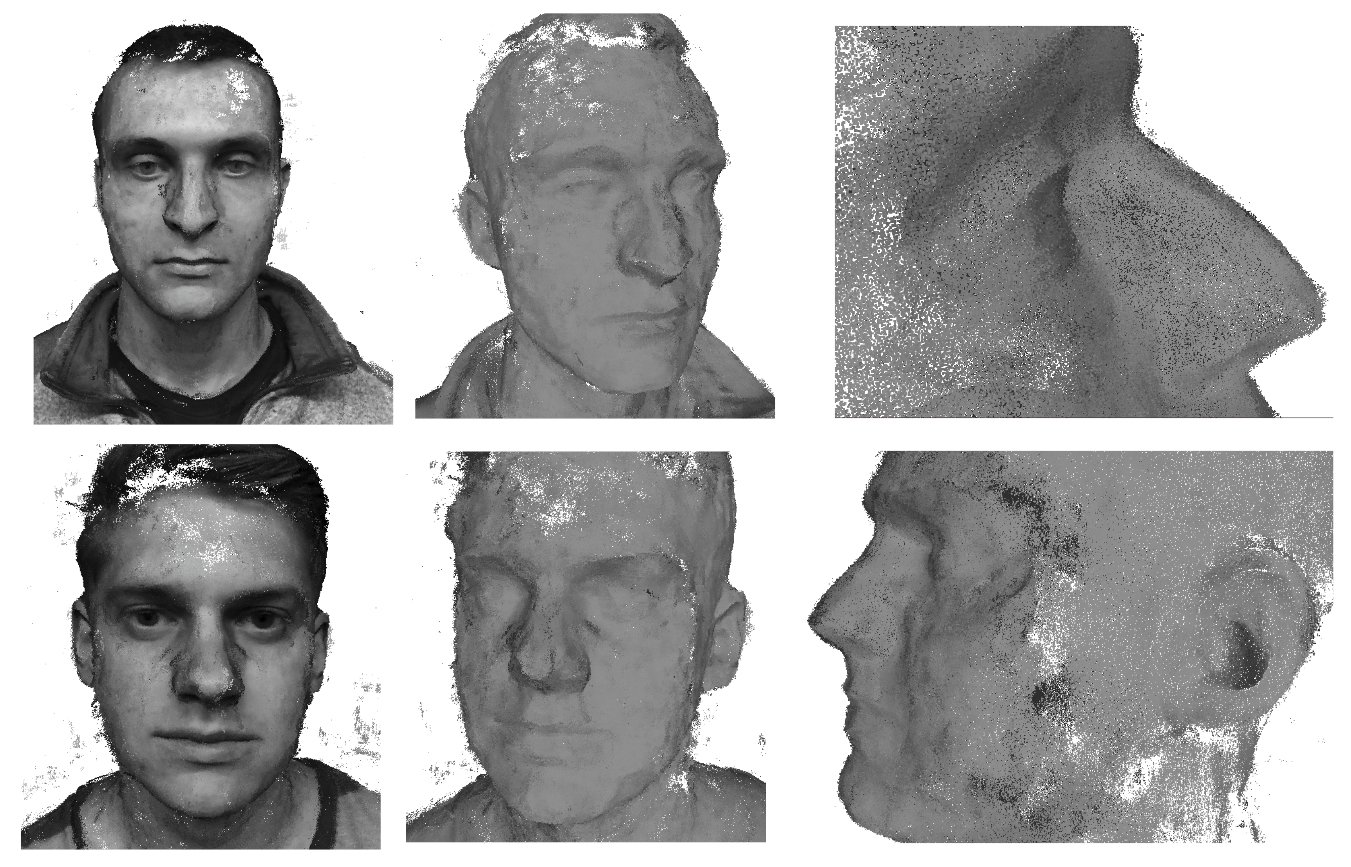
\includegraphics[width=0.95\linewidth]{images/point_clouds_sample.png}
\end{center}
   \caption{Example point clouds generated at the end of our Point cloud generation stage, with and without texture. The point clouds accurately capture the overall face geometry and a lot of details in areas like eyes and lips, that make the person recognizable. However, the point clouds have missing data as well as noise, which requires a robust mesh fitting approach, discussed in Section \ref{sec:mesh_fit}.  }
\label{fig:pcl_sample}
\end{figure}

%-------------------------------------------------------------------------
\subsection{Mesh fitting} \label{sec:mesh_fit}


Due to factors like non-ideal lighting, lack of texture and sensor noise of the smartphone, the obtained point cloud typically has noise and incompletions, with the points distributed around the `true' surface.
 Techniques like Screened Poisson reconstruction or the depth map fusion strategy of \cite{hernandez2015near} either return meshes with a lot of surface noise, or extremely smoothed out details, depending on the regularization used (see Fig. \ref{fig:mesh_comp}). Further, for the reconstructed mesh to be of use in further downstream tasks such as animation, bio-metrics or as input to a learning algorithm, it is extremely desirable for the meshes to have a consistent topology. \\
 \begin{figure}[t]
\begin{center}
   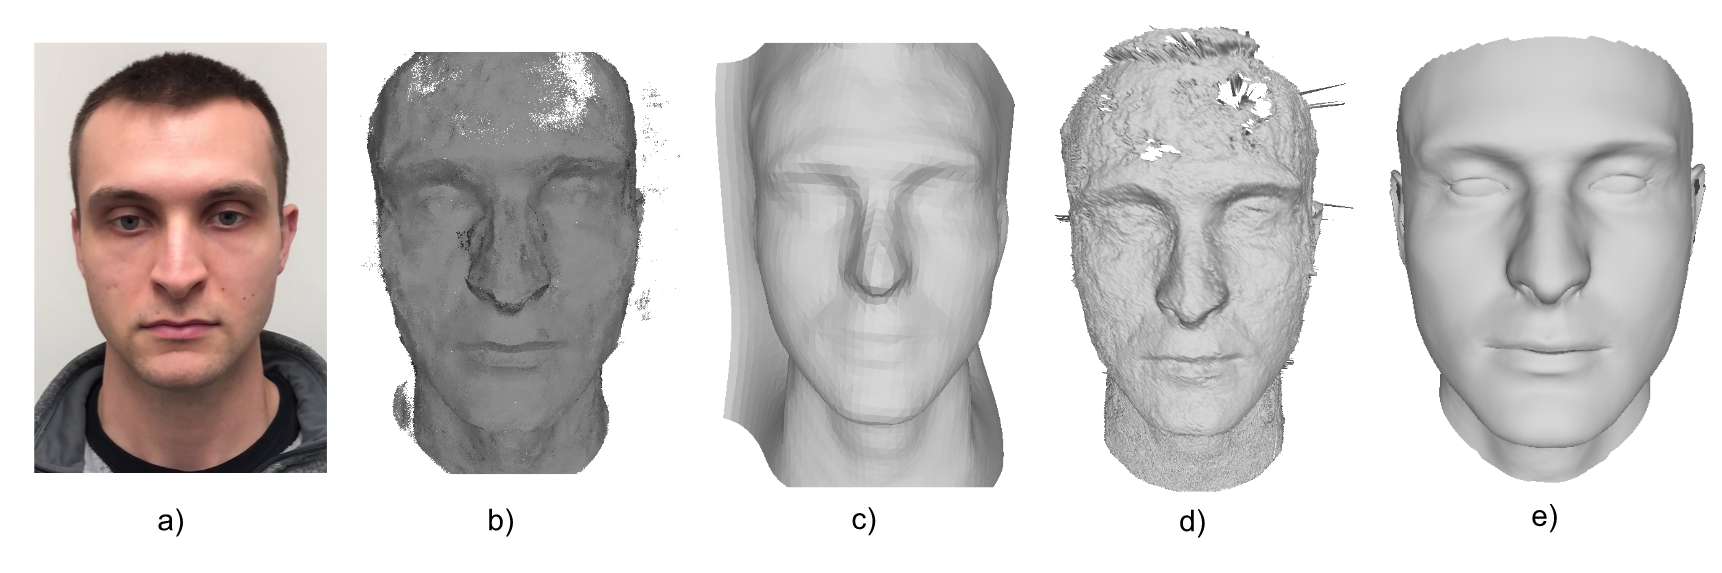
\includegraphics[width=0.95\linewidth]{images/meshing_compare.png}
\end{center}
   \caption{Comparison of mesh generation methods from the reconstructed point cloud. a) Sample image. b) Generated point cloud. c) Screened Poisson Surface Reconstruction \cite{kazhdan2013screened} can fill in gaps in the point cloud but at the cost of overly smooth meshes. d) The depth fusion strategy proposed in \cite{hernandez2015near} can preserve details, but is unable to handle missing data. e) Our approach reconstructs meshes with consistent topology and correspondence between vertices, while capturing details of the point cloud and being robust to noise and missing data. }
\label{fig:mesh_comp}
\end{figure}

 Statistical ICP inspired techniques have proposed fitting a 3DMM to a point cloud \cite{schneider2009fitting,bazik2017robust,blanz2004statistical} in the past. However, they often assume that the point cloud obtained from an RGB-D sensor is `clean'. Further, fitting a 3DMM defeats the purpose of not being constrained to an existing linear basis of shape.
 We thus adapt the non-rigid mesh fitting algorithm of \cite{amberg2007optimal}, originally proposed for registering template meshes to 3D scanner data, to deform a template using a combination of constraints given by the point cloud, landmarks, mesh stiffness and edge constraints. 
 
 
 \subsubsection{Point cloud constraints}
 The primary constraint for the mesh deformation comes from the 3D information captured in the point cloud.
 While well studied techniques exist to register a template mesh to a 3D scanned mesh \cite{amberg2007optimal}, registering a mesh to point clouds of the sort obtained from multi-view stereo techniques is more challenging. For example, simply fitting each vertex to its nearest-neighbor in the point cloud will cause the mesh to become extremely noisy, as there will be many outlier points.
 
To address this, we take advantage of the fact that for a template mesh, the vertex normals can be easily estimated. For each vertex, we select the points in its neighborhood, and for each point, we calculate its perpendicular distance to the normal of the vertex. Points within a small threshold distance are accepted while the rest are rejected (see Fig. \ref{fig:mesh_fit_pcl}. 
 
 For each vertex on the template mesh we obtain its desired location in 3D as the median of the accepted points. \\
 
\begin{figure}[t]
\begin{center}
   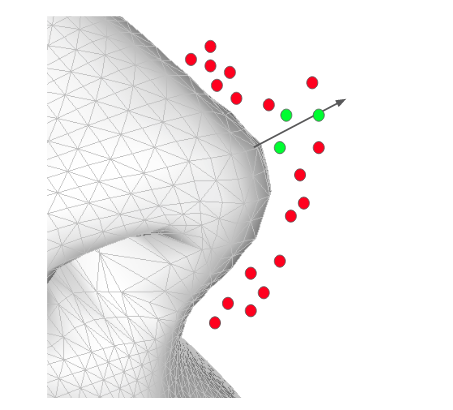
\includegraphics[width=0.8\linewidth]{images/mesh_fit_pcl.png}
\end{center}
   \caption{Exaggerated view of the point cloud fitting. For each vertex, the set of points within a small threshold of its normal (in green here) are found and their median used as the target 3D coordinate for the vertex. }
\label{fig:mesh_fit_pcl}
\end{figure}

 
 \subsubsection{Landmark constraints}

 The second source of information are the 68 2D landmarks obtained using the automatic landmarking solution of \cite{baltrusaitis2018openface}. Landmarks are important for global alignment and scaling of the mesh, as well as ensuring all the reconstructed meshes are in semantic correspondence.
 
 For the set of frames for which the landmarks have been annotated with high confidence by the tracker (typically close to frontal poses), we solve for the 3D locations of the landmarks by minimizing geometric reprojection error, 
 \begin{equation}
    E_{X_{j}} = \sum_{i} \sum_{j} d(\pi (\theta_{i},X_{j}),x_{ij})^2
\end{equation}
Where $\theta_i$ is the $i$-th camera's pose, $X_{j}$ is the $j$-th landmark's coordinates in 3D, and $x_{ij}$ is the 2D coordinate of the landmark returned by the landmark tracker for the $i$-th frame. For our purposes, we ignore the 18 landmarks corresponding to the face contour, and use the remaining 50 landmarks as additional constraint for the corresponding 3D vertices.\\


Historically, most landmark trackers have focused only on these 68 key-points. As a consequence, many reconstruction techniques either focus only on reconstructing the frontal face region, or generate a full mesh but evaluate only on the frontal section. Ears and the side facial regions have mostly been ignored in previous works. Even learning-based face alignment techniques do not do well on the ears, as the underlying training data is based on the the annotation/detection of these 68 landmarks.

To explicitly address this, we make use of a recent dataset of `in-the-wild' ear images annotated with bounding boxes and landmarks \cite{zhou2017deformable}. We first train the deep object detection model of Redmon \etal \cite{redmon2017yolo9000} for a single `ear' class. We then train an ensemble of regression trees \cite{kazemi2014one} for predicting landmarks using the bounding box detection as input. As seen in Fig \ref{fig:ear_lm_and_edges}, despite the limited training data size, we are able to achieve impressive robustness and accuracy in the landmark detection. We use a subset of the landmarks corresponding to the outer contour of the ear as additional landmark constraint in our mesh fitting. To the best of our knowledge, ours is the first face reconstruction method to explicitly address the ears, which in turn improves overall accuracy and metrics like the width of the face.

\begin{figure}[t]
\begin{center}
   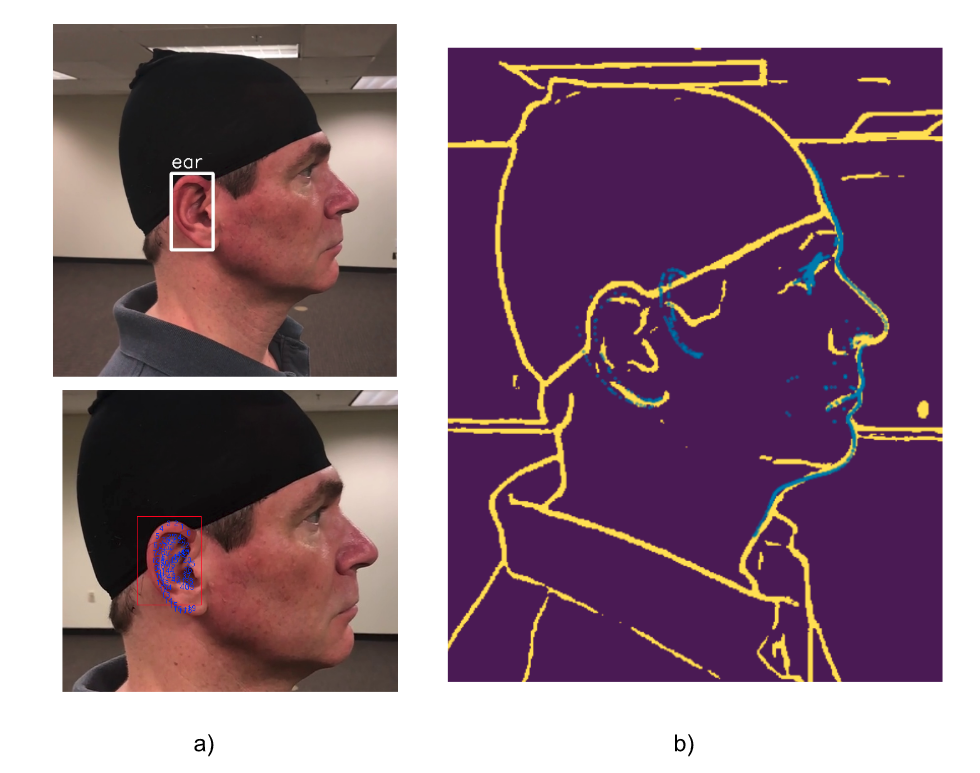
\includegraphics[width=0.95\linewidth]{images/ear_lm_and_edges.png}
\end{center}
   \caption{ a) We train a bounding box regressor (above) and landmark detector (below) specifically for ears. This improves our reconstruction's overall accuracy while allowing us to capture ear size and contour. b) Visualization of edge constraints. Edges in RGB image are shown in yellow, mesh vertices projected in blue. Note that our mesh fits the ears well because of the landmark detection }
\label{fig:ear_lm_and_edges}
\end{figure}





\subsubsection{Edge constraints}
Silhouette constraints have shown to be powerful cues in recent 3D reconstruction literature \cite{alldieck2018detailed,bas2016fitting}. For faces, views that are close to profile are particularly informative. However, since many single and multi-view approaches rely on landmarking for camera pose estimation, they fail to make use of silhouettes beyond a certain angle.
As mentioned in Sec \ref{sec:PBA}, by solving for the camera poses independently of landmarking, we can actually make use of extreme profile views. This is helpful as they contain a lot of information for areas that have typically proven to be challenging for face reconstruction algorithms, such as the nose, lips and lower chin/neck region.
We use a combination of Z-buffering \cite{Foley1990ComputerG} and backface-culling  to estimate vertices that project an edge onto a given view. To find the corresponding edges in the RGB image, we use the Structured Forests edge detection approach proposed in \cite{dollar2013structured}. For each vertex projecting an edge in the frame, its nearest neighbour is found in the edge map. This corresponding point is backprojected in 3D to obtain a `target' location for the vertex in 3D.


 \subsubsection{Putting it all together}
 With the combination of the cues from the point cloud, keypoints and silhouettes, we obtain a set of mapping from the template mesh vertices (source) to coordinates in 3D (target). This can then be expressed in the iterative linear system-based non-rigid mesh registration algorithm proposed by Amberg \etal \cite{amberg2007optimal}. 
 
 At each iteration, a linear system of the form $\mathbf{A}\mathbf{X} = \mathbf{B}$ is solved, where $\mathbf{X}$ is a $4n\times4$ matrix, the per-vertex 4x4 transform matrix. The matrix $\mathbf{A}$ captures information of the source template, in terms of the mesh connectivity and vertex locations. The mesh connectivity acts as an adjustable `stiffness' regularization, which controls how much neighboring vertices can move with respect to each other. The matrix 
 $\mathbf{B}$ contains the corresponding `target' locations in 3D. The mesh stiffness and the weights of the landmarks are gradually decreased, gradually moving from global stretching to local, data driven deformations. After every few iterations, the point cloud and edge constraints are recalculated using the current locations of the vertices. For further details we refer the reader to the original paper \cite{amberg2007optimal}. For our template, we use the Basel 3DMM mesh \cite{blanz1999morphable}, simply because of its prevalence as an input or output of several face reconstruction algorithms.

% \begin{table}
% \begin{center}
% \begin{tabular}{|l|c|}
% \hline
% Method & Frobnability \\
% \hline\hline
% Theirs & Frumpy \\
% Yours & Frobbly \\
% Ours & Makes one's heart Frob\\
% \hline
% \end{tabular}
% \end{center}
% \caption{Results.   Ours is better.}
% \end{table}

%---------------------------



%------------------------------------------------------------------------
%------------------------------------------------------------------------
%-------------------------------------------------------------------------
%------------------------------------------------------------------------

\section{Results}

We collect a dataset of videos of subjects using an iPhone X. . Each sequence is 15-20 seconds long 

Describe input video, recorded with iphoneX 

%%%%%%%%%%%%%%%%%%%%%%%%%%%%%%%%%%%%%%%%%%%%%%%%%%%%%%%%%%%%%%%%%%%%%%%%%%%%%%55
%%%%%%%%%%%%%%%%%%%%%%%%%%%%%%%%%%%%%%%%%%%%%%%%%%%%%%%%%%%%%%%%%%%%%%%%%%%%%%%%5
\subsection{Quantitative Evaluation} \label{sec:quant}

For 10 subjects among the videos we collected, we obtained high accuracy 3D face scans using an Arctic Eva structured light hand-held scanner. The scans were obtained immediately after the video was recorded with the subjects still in the same poses, to ensure no discrepancy in face geometry between the video and the scan. We use the videos of these subjects to reconstruct face meshes using the methods listed in Table \ref{table:results}. For methods that work on a single image, we use a close to frontal keyframe as input. For the edge-fitting based single view method of Bas \etal \cite{bas2016fitting}, we select a frame at roughly 15 degrees to the front for the input, since that was reported to work best in their paper. For the multi-view methods, we either use the keyframes generated by our method or the whole video, depending on what the method uses as input.
% However the methods of Roth \etal and PCSfM are not able to make use of all of our keyframes as they are reliant on landmark detectors for alignment and pose estimation, and so typically only use frames in a cone around the front of the face. For the method of multi-view landmark fitting, we use the whole video, using the implementation provided in 4dface \cite{huber2016multiresolution}). 
For all methods except PCSfM, the authors make their implementations public and we use those for evaluation. For PCSfM, we use our own implementation.

A challenge in fair quantitative evaluation arises from the fact that different methods reconstruct different amounts of the face area as defined by the Basel mesh, such as frontal only in pix2vertex \cite{sela2017unrestricted} , front and side without ears in PRN \cite{feng2018joint}, full Basel mesh for PCSfM \cite{hernandez2017accurate} and arbitrary in SfM (using COLMAP \cite{schonberger2016structure}). To address this, we first register a standard Basel mesh to the ground truth 3D scans using Non-rigid ICP \cite{amberg2007optimal,booth2018large}. Then, borrowing a strategy from MVS benchmarks \cite{jensen2014large,knapitsch2017tanks,yao2018mvsnet}, we evaluate the reconstructions using \textbf{Accuracy} - the mean distance from the reconstruction's vertices to the ground truth, and \textbf{Completion} - the mean distance from the ground truth's vertices to the reconstruction. Thus, if a method reconstructs only the frontal face, it might do well in Accuracy and be penalized in Completion.

\textbf{Ablation.} Without edges, without ear landmarks

All numbers are in millimeters. As noted in \cite{hernandez2017accurate}, meshes with smooth areas tend to make the numeric error lower, even if the reconstruction does not really resemble the ground truth.


%%%%%%%%%%%%%%%%%%%%%%%%%%%%%%%%%%%%%%%%%%%%%%%%%%%%%%%%%%%%%%%%%%%%%%%%%%%%%%%%%%%%%%%%%%%%%%%%%%%%%%%%%%%%%
%%%-------------------------------MAIN TABLE------------------------------------------------------------------------

\begin{table*}
\begin{center}
\begin{tabular}{|c|c|c c c|c c c|}
\hline 
\multirow{2}{*}{Method} & \multirow{2}{*}{Views} 
& \multicolumn{3}{c|}{Accuracy (mm) $\downarrow$} 
& \multicolumn{3}{|c|}{Completion(mm) $\downarrow$} \\ 
\cline{3-8}
& & Mean & Std. Dev. & Median & Mean & Std. Dev. & Median\\
\hline\hline
Mean Basel \cite{blanz1999morphable}       & -        & 3.2  & &     & 0.775    & & \\ 
Landmark fitting \cite{huber2016multiresolution}  & Single  & 2.6  & & & 0.766     & &     \\ 
pix2vertex \cite{sela2017unrestricted} & Single & 3.32 & & & 11 & &  \\
PRN \cite{feng2018joint} & Single & 3.1 & & & 8 & & \\
Edge-fitting \cite{bas2016fitting} & Single & 2.7 & & & 6 & & \\

\hline
M.view lm fit \cite{huber2016multiresolution,huber2015fitting} & Multi   & 1.89 & &       & 0.746          & &   \\ 
Roth \etal \cite{roth2015unconstrained}     & Multi      & 2.741 & & & 3 & & \\
SfM \cite{schonberger2016structure} & Multi & 5.4 & & & 1.7 & & \\
PCSfM* \cite{hernandez2017accurate} & Multi & 2.34 & & & 2.2 & & \\
\hline
Ours w/o Edges    &  Multi  & 1.378 & & & 1.472 & &     \\
Ours w/o ear lms    &  Multi     & 1.320 & & & 1.045 & &      \\
Ours    &  Multi     & 1.273 & & & 0.977 & &     \\

% \specialrule{.16em}{.08em}{.081em}
\hline
\end{tabular}
\end{center}
\caption{Quantitative results against ground truth scans. We evaluate the state of the art single and multi-view reconstruction methods. As is common in MVS benchmarks, we evaluate the reconstructions in terms of average distance from reconstruction to ground truth (accuracy) and distance from ground truth to reconstruction (completion). All numbers in mm; lower is better. * denotes that the method needs camera intrinsics to be known in advance.}
\label{table:results}
\end{table*}



% \begin{table*}[t]
% \centering
% \caption{Quantitative results against ground truth scans. We evaluate the state of the art single and multi-view reconstruction methods. As is common in MVS benchmarks, we evaluate the reconstructions in terms of average distance from reconstruction to ground truth (accuracy) and distance from ground truth to reconstruction (completion). All numbers in mm; lower is better. * denotes that the method needs camera intrinsics to be known in advance.}
% % \resizebox{\textwidth}{!}{%


% \begin{tabular}{c |c| c | c c c}
% \hline
% Method & Views & Accuracy & Completion & Consistency \\
% \hline\hline
% Mean Basel \cite{blanz1999morphable}       & -        & 3.2       & 0.775          & 0 \\ 
% Landmark fitting \cite{huber2016multiresolution}  & Single  & 2.6          & 0.766      & 0.1    \\ 
% pix2vertex \cite{sela2017unrestricted} & Single & 3.32 & 11 & - \\
% PRN \cite{feng2018joint} & Single & 3.1 & 8 & - \\
% Edge-fitting \cite{bas2016fitting} & Single & 2.7 & 6 & - \\

% \hline
% M.view lm fit \cite{huber2016multiresolution,huber2015fitting} & Multi   & 1.89        & 0.746          & 75.73  \\ 
% Roth \etal \cite{roth2015unconstrained}     & Multi      & 2.741 & 3 & - \\
% SfM \cite{schonberger2016structure} & Multi & 5.4 & 1.7 & - \\
% PCSfM* \cite{hernandez2017accurate} & Multi & 2.34 & 2.2 & -\\
% \hline
% Ours w/o Edges    &  Multi  & 1.378 & 1.472 & -     \\
% Ours w/o ear lms    &  Multi     & 1.320 & 1.045 & -      \\
% Ours    &  Multi     & 1.273 & 0.977 & -     \\

% % \specialrule{.16em}{.08em}{.081em}
% \hline
% \end{tabular}%
% % }
% \label{table:results}
% \end{table*}
%%%%%%%%%%%%%%%%%%%%%%%%%%%%%%%%%%%%%%%%%%%%%%%%%%%%%%%%%%%%%%%%%%%%%%%%%%%%%%%%%%%%%%%%%%%%%%%%%%%%%%%%%%

\begin{figure*}
\begin{center}
   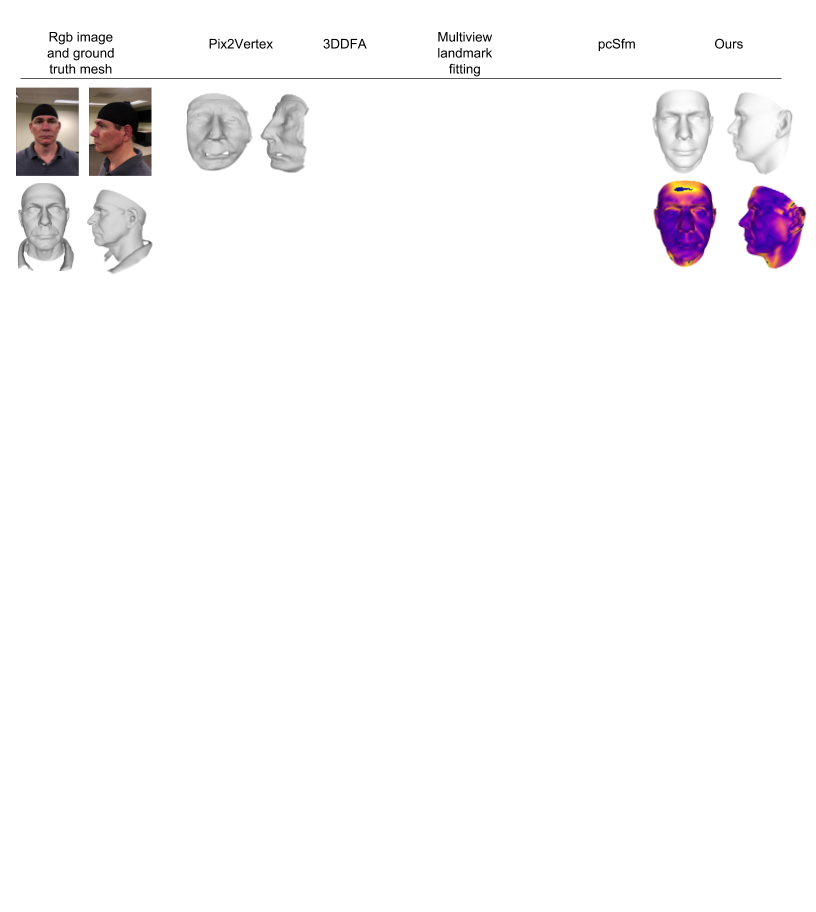
\includegraphics[width=0.95\linewidth]{images/ICCV_verticals.png}
\end{center}
  \caption{Reconstruction and error heat map visualization of various approaches}
\label{fig:results}
\end{figure*}

%%%%%%%%%%%%%%%%%%%%%%%%%%%%%%%%%%%%%%%%%%%%%%%%%%%%%%%%%%%%%%%%%%%%%%%%%%%%%%%%%%%%%5
%%%%%%%%%%%%%%%%%%%%%%%%%%%%%%%%%%%%%%%%%%%%%%%%%%%%%%%%%%%%%%%%%%%%%%%%%%%%%%%%%%%5%%


\subsection{Qualitative evaluation} \label{sec:qual}
\begin{figure}[t]
\begin{center}
% \fbox{\rule{0pt}{2in} \rule{0.9\linewidth}{0pt}}
   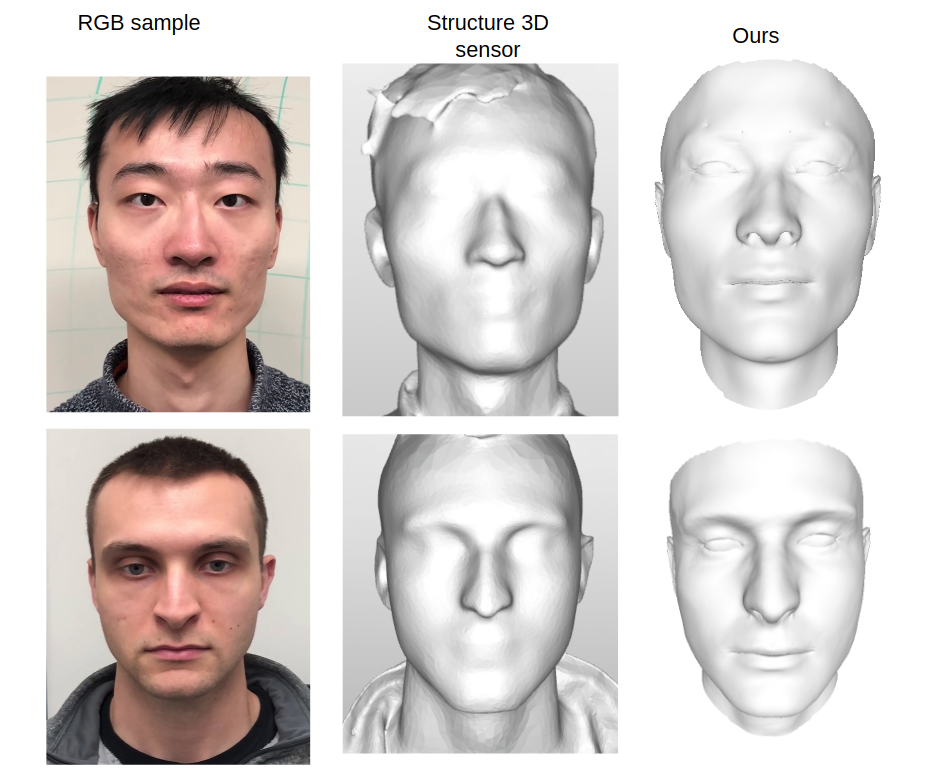
\includegraphics[width=0.9\linewidth]{images/struc_3d_comp.png}
\end{center}
   \caption{Our method reconstructs meshes with more detail than a Structure Sensor, a commercially available low cost IR-based RGB-D scanner \cite{structure2019} specialized for scanning humans. As can be seen, details like the eyes, nose and lips are excessively smoothed out.}
\label{fig:long}
\label{fig:onecol}
\end{figure}

Compare against scan obtained by structure 3d sensor -> comment on better than low cost depth sensor, while being eeve easier for the end user.

\subsubsection{Expressions}

 \begin{figure}[t]
\begin{center}
   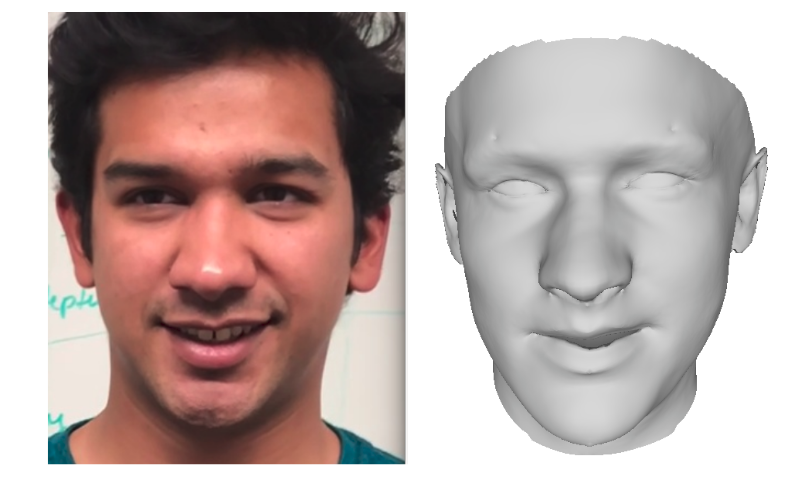
\includegraphics[width=0.8\linewidth]{images/expression_dummy.png}
\end{center}
   \caption{ TEMP, DONT PUT SELF FACE- COLLECT other scans from lab, potentially push to supplementary }
\label{fig:expressions}
\end{figure}

Since our method captures the geometry of the face in a completely data-driven manner, it also generalizes to deformations caused by expressions. 
Since it is difficult to hold the same expression through a video sequence and also obtain a corresponding ground truth 3D, we skip quantitative evaluation of this and provide some qualitative visualizations in Fig \ref{fig:expressions}. 
We also note that since there is dense correspondence and consistent topology across meshes, various existing techniques \cite{}  anchor frames, rigging, animation, blendshapes/warehouse, can be applied with our reconstructed meshes to generate animated, expressive face models.


\subsubsection{Fine detail enhancement}
A recent trend in the 3D face reconstruction community has been to emboss fine high frequency details to the reconstruction using techniques like shape-from-shading or mesoscopic augmentations using texture cues. While not always reflecting the true geometry of the surface, these methods add realism to the mesh, which can be desirable for purposes like animation. Such methods can easily be applied to our reconstructions as well.\\
Recently Sela \etal\cite{sela2017unrestricted} showed impressive results by interpreting the idea of high frequency mesoscopic augmentations \cite{beeler2010high} through mesh heat flows. In our experiments we found this method to not adapt well to ``in-the-wild" images, distorting the mesh too much due to sensor noise/unconstrained lighting. We make some modifications to their method to add details without losing the underlying mesh structure. 
Since this method is based on a "dark-is-deep" assumption and not necessarily founded in geometry, we skip quantitative evaluation for these results and simply provide qualitative comparisons between our reconstructions, with and without our augmentation scheme, compared to the augmentation scheme of \cite{sela2017unrestricted}. Details on the modifications made are provided in the supplementary.
% \begin{itemize}
%     \item Previous work on "dark-is-deep" assumption. Mention learnt mesoscopic and studio requirement
%     \item Mention i2i mesh heat flow for high pass, we propose band pass formulation 
%     \item Capture medium scale detail by deforming directly with difference from mean
% \end{itemize}

%%%%%%%%%%%%%%%%%%%%%%%%%%%%%%%%%%%%%%%%%%%%%%%%%%%%%%%%%%%%%%%%%%%%%%%%%%%%%%%%%
%%%%%%%%%%%%%%%%%%%%%%%%%%%%%%%%%%%%%%%%%%%%%%%%%%%%%%%%%%%%%%%%%%%%%%%
\section{Dataset}
\begin{table}
\begin{center}
\begin{tabular}{|l|c| c|}
\hline
Dataset & \# Subjects & \# Poses \\
\hline\hline
ND-2006 & 888 & None \\
BU-3DFE & 100 & 2 \\
Texas 3DFRD & 118 & None\\
Bosphorus & 105 & 13\\
CASIA-3D & 123 & 11\\
MICC & 53 & Multi*\\
UHDB11 & 23 & 12\\
\hline
\end{tabular}
\end{center}
\caption{An overview of available 3D face datasets and the pose variation in RGB images available in them. Note that although MICC contains videos of subjects with varying pose, the subjects do not hold the same expression through the video, so ground truth for most views is not available}
\end{table}


\begin{itemize}
    \item  Limited 3d gt data, our experiments reveal severe flaw of deep learning methods trained on synthetic data (pix2vertex), showing very poor generalization to true "in-the-wild" images, with different lighting/noise models then what was use to generate the synthetic data. 
    \item Validated on subset for which ground truth obtained using high accuracy structured light. Rest of the scans are validated using "self-consistency" : for the two sequences of a subject collected under different conditions, the resulting meshes are ensured to be similar up to a tolerance.
    \item Help more interesting deep learning : cite mvsnet / dtu dataset
    \item We provide video, reconstructed mesh and 50-100 "keyframes" with known camera poses with respect to the mesh, We also provide the depth map and surface normal map obtaine dusing the mesh
    \item We hope "In the wild" , unconstrained , help train and evaluate robust yet accurate and consistent multi and single view reconstruction algorithms

    \item repeat synthetic data problem, refer to results/images
    \item Self validate others, different lighting conditions

\end{itemize}

\section{Conclusion}
Limitations, importance to community

\newpage
\newpage
{\small
\bibliographystyle{ieee}
\bibliography{egbib}
}




\end{document}
